\documentclass[a4paper,10pt]{article}

% Hier die Nummer des Blatts und Autoren angeben.
\newcommand{\blatt}{12}
\newcommand{\autor}{Ralf Engelken, Joachim Schmidberger, Frank Woithe, Michael Steinke, Merlin Koglin}

\usepackage{hci}
\usepackage{float} 

\begin{document}
% Seitenkopf mit Informationen
\kopf
\renewcommand{\figurename}{Figure}

\aufgabe{17 \textit{(Team-Aufgabe)}} 
\begin{enumerate}
\item Analyse

PACT-Analyse

\begin{enumerate}
\item Personen\\
Britta Behrens
\begin{itemize}
\item Alter: 28
\item Beruf: Fahrzeugbau-Ingenieurin
\item Motto: Wenn es nicht fährt, baue einen Antrieb ein
\item Hobbies: Bastelt gerne elektrische Geräte zusammen
\item Persönlichkeit: Hat gern über alles Kontrolle und möchte viel Einstellen können. Möchte immer die neusten technischen Gadgets haben.
\end{itemize}

Stefan Schmidt
\begin{itemize}
\item Alter: 34
\item Beruf: Kaufmann
\item Motto: Nur nicht zu kompliziert
\item Hobbies: Sport, Reisen
\item Persönlichkeit: mag unkomplizierte und zuverlässige Geräte
\end{itemize}

\item Aktionen

\begin{itemize}
\item Der Benutzer startet die vorbereitete Waschmaschine/Kaffemaschine, sodaß die Wäsche/der Kaffee fertig ist, wenn er nach Hause kommt.
\item Der Benutzer schaltet die Heizung ein, damit es warm ist, wenn er nach Hause kommt.
\item Der Benutzer programmiert den Videorekorder, um eine Sendung aufzuzeichnen.
\item Der Benutzer kann Fenster und Rollläden öffnen/schließen und das Licht steuern.
\item Der Benutzer kann die Bewässerungsanlage steuern.
\item Der Benutzer kontrolliert per Überwachungskamera, ob der Hund Wache hält oder schläft.
\item Der Benutzer kann den Mixer einschalten, um den Gremlin zu erledigen, der in der Küche herumschleicht.
\end{itemize}

\item Kontext

\begin{itemize}
\item Das Gerät wird am Handgelenk getragen
\item die Bedienung erfolgt oft ohne feste Unterlage, evtl. im Gehen (ungenaue Bedienung)
\item die Bedienung erfolgt unter verschiedensten Lichtverhältnissen
\item eventuelle unbeabsichtigte Eingaben (z.B. Kleidung scheuert über die Uhr)
\end{itemize}

\item Technologie

\begin{itemize}
\item Eingaben erfolgen über das Touch-Display
\item Ausgabe über Display (evtl. Töne, Vibration?) oder über das verbundene Smartphone
\end{itemize}

\end{enumerate}

\newpage
\item Design

\begin{figure}[H]
	\centering
	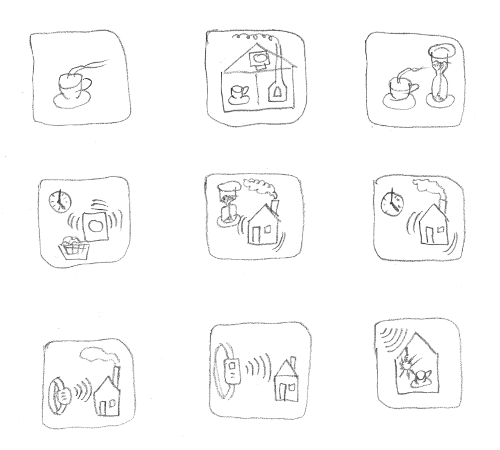
\includegraphics[width=0.8\textwidth]{Sketches_Icon.png} 
	\caption{Sketches Icon}
	\label{fig1}
\end{figure}
\begin{figure}[H]
	\centering
	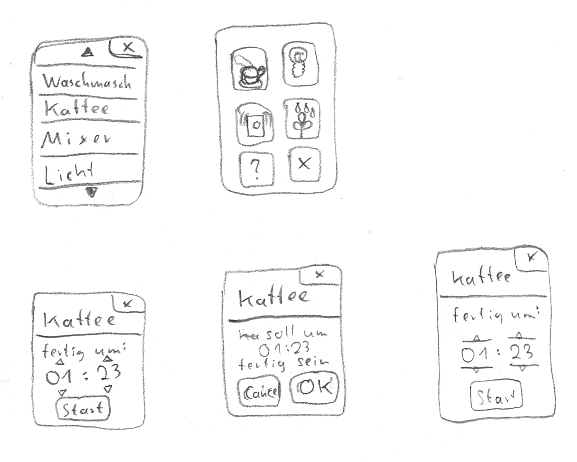
\includegraphics[width=0.8\textwidth]{Sketches_App.png} 
	\caption{Sketches App}
	\label{fig2}
\end{figure}

\newpage
\item Implementierung
Für die Bedienung wurde das "Hub and Spoke"-Pattern gewählt. Vom Hauptmenü aus können voneinander unabhängige Untermenüs erreicht werden. Im Prototypen wurde das Hauptmenü durch eine scrollbare Menuleiste realisiert. So kann man die App leicht erweitern, wenn im Smart Home weitere steuerbare Elemente hinzukommen.

Wenn man im Hauptmenü den Menüpunkt Kaffemaschine auswählt, kommt man auf die Auswahlseite für die Zeit. Dort kann man die Zeit einstellen, zu der der Kaffee aufgebrüht werden soll. Man kann die Zeit einstellen und die Programmierung per Start abschließen oder per Cancel abbrechen und ins Hauptmenü zurückkehren. Per default wird das aktuelle Datum gesetzt, per Swipe kommt man zum Datums-Menü, in dem man das Ziel-Datum ändern kann, und zu den Optionen, in denen man den kaffee konfigurieren kann. Von jedem Punkt des Swipe-Menüs kann man die Programmierung beenden oder abbrechen.
\begin{figure}[H]
	\centering
	\includegraphics[width=0.5\textwidth]{Screenshot-Hauptmenü.png} 
	\caption{Prototyp: Hauptmenü}
	\label{fig3}
\end{figure}
\begin{figure}[H]
	\centering
	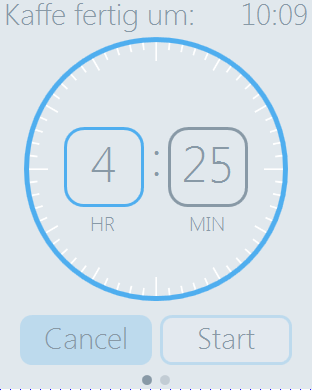
\includegraphics[width=0.5\textwidth]{Screenshot-AuswahlZeit.png} 
	\caption{Prototyp: Auswahl der Zielzeit}
	\label{fig4}
\end{figure}
\begin{figure}[H]
	\centering
	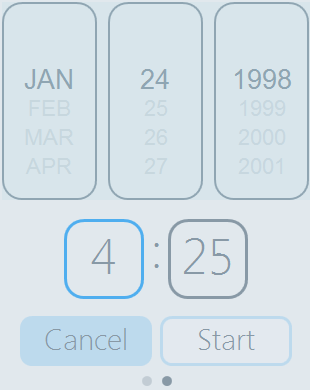
\includegraphics[width=0.5\textwidth]{Screenshot-AuswahlDatum.png} 
	\caption{Prototyp: Auswahl des Zieldatums}
	\label{fig5}
\end{figure}
\begin{figure}[H]
	\centering
	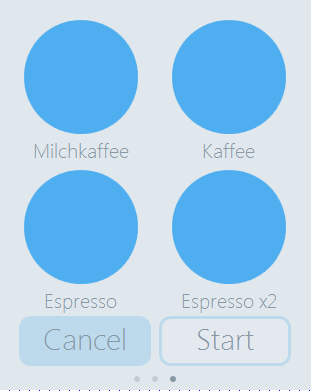
\includegraphics[width=0.5\textwidth]{Screenshot-AuswahlOptionen.png} 
	\caption{Prototyp: zusätzliche Optionen}
	\label{fig5}
\end{figure}

\newline
\item Evaluation
Wir konnten die Mixersteuerung leider nicht testen, da wir keine Gremlins auftreiben konnten. Wir sind jedoch sicher, daß die Fernsteuerung eine signifikante Verbesserung darstellt, da die Anwesenheit in der Küche beim Starten des Mixers etreme gesundheitliche Riskien mit sich bringt.

\end{enumerate}
\end{document}
